\chapter{Data acquisition}

The data used in the paper has been gathered over the course of three months, starting in early March and ending in late May. The data has been obtained with the help of three student volunteers. Each volunteer carried a phone, provided by the SensibleDTU project, the same project this thesis is a part of \cite{sensibledtu, Stopczynski}. The phones are Samsung Galaxy Nexus \cite{nexus} and are running the Android operating system \cite{android}.

Each phone came with two apps. The first recorded regularly a multitude of information, such as Bluetooth RSSI, GPS traces, battery usage and cell tower information, and is a part of the SensibleDTU project \cite{Stopczynski}, while the second allowed the volunteers to manually name the person they are in physical proximity with, and was developed during this thesis. The second app provided the ground-truth information that confirmed the existence of physical proximity.

This gave rise to two types of data. First, a continuous stream of regular measurements from the first app, and punctual messages from the second app. Below we will go into more detail about how exactly the two types of data look, how are they gathered and finally, how the two are combined to create a unitary set which serves as a basis for the machine learning algorithms.

One last thing to mention is that the volunteers were not chosen completely random, but in such a way that guaranteed the existence of both types of data. On the one hand, the volunteers are all studying for a computer science major at DTU. This ensured that the students have found themselves in each others vicinity at some point during the data gathering period. Also, all three volunteers live in different places. This is important because house-mates or couples living together will introduce a very large amount of data that is very specific, while we are looking to generalize as much as possible.
On the other hand, we needed to make sure that eventually, some volunteers are in each other's physical proximity. This was resolved by the fact that the volunteers had a course together. This ensured that at least once per week, usually two because of group work, the volunteers met.

\section{Bluetooth}

\section{FriendFinder app}

\subsection{App overview and implementation}

As the app, FriendFinder, is made for the Android operating system, it is implemented using Java for Android \cite{jandroid}. It has a Google App Engine backend \cite{googleapp}. Fig \ref{pic:ff_prtscr} shows the main screen of the app. 

\begin{figure}[h]
	\begin{center}
		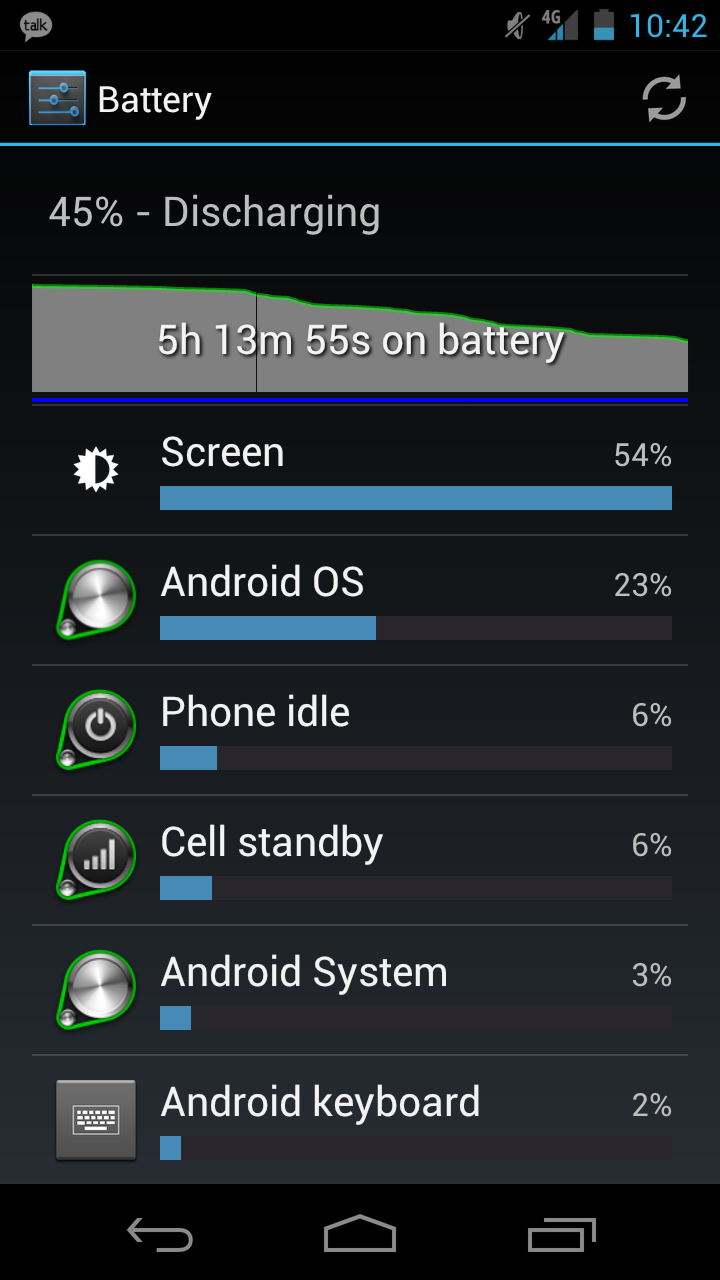
\includegraphics[scale=0.2]{figures/galaxy-nexus-battery.png}
	\end{center}
	
	\caption{FriendFinder app}.
	\label{pic:ff_prtscr}

\end{figure} 

FriendFinder is implemented using a client server architecture, where the clients are the apps installed on the phone, and the server is the Google App Engine. Fig \ref{pic:clientserver} shows an overview of this particular architecture. In this case, the FriendFinder app (in the role of the client) makes a \textit{save data} request to the Google App Engine (the server). The server in turn responds with the result of the operation, either a \textit{succes} or \textit{failure} message.  

\begin{figure}[h]
	\begin{center}
		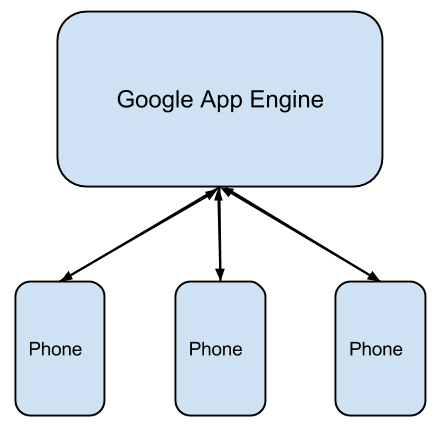
\includegraphics[scale=0.5]{figures/SC_Arch.png}
	\end{center}
	
	\caption{Client Server Architecture used by the FriendFinder app}.
	\label{pic:clientserver}

\end{figure} 

The app contains a single screen (the one showed in Fig \ref{pic:ff_prtscr}), which corresponds to the main activity. Activities are the main building blocks of an Android app, and they are used both to interact with the user, as well as provide additional functionalities \cite{activity}. On the main screen there are buttons for each volunteer. Once one of the volunteers is in physical proximity with another volunteer (as perceived by either one), they both press the button corresponding to each other. A confirmation message is displayed, as can be seen in Fig. \ref{pic:ff_conf}.

\begin{figure}[h]
	\begin{center}
		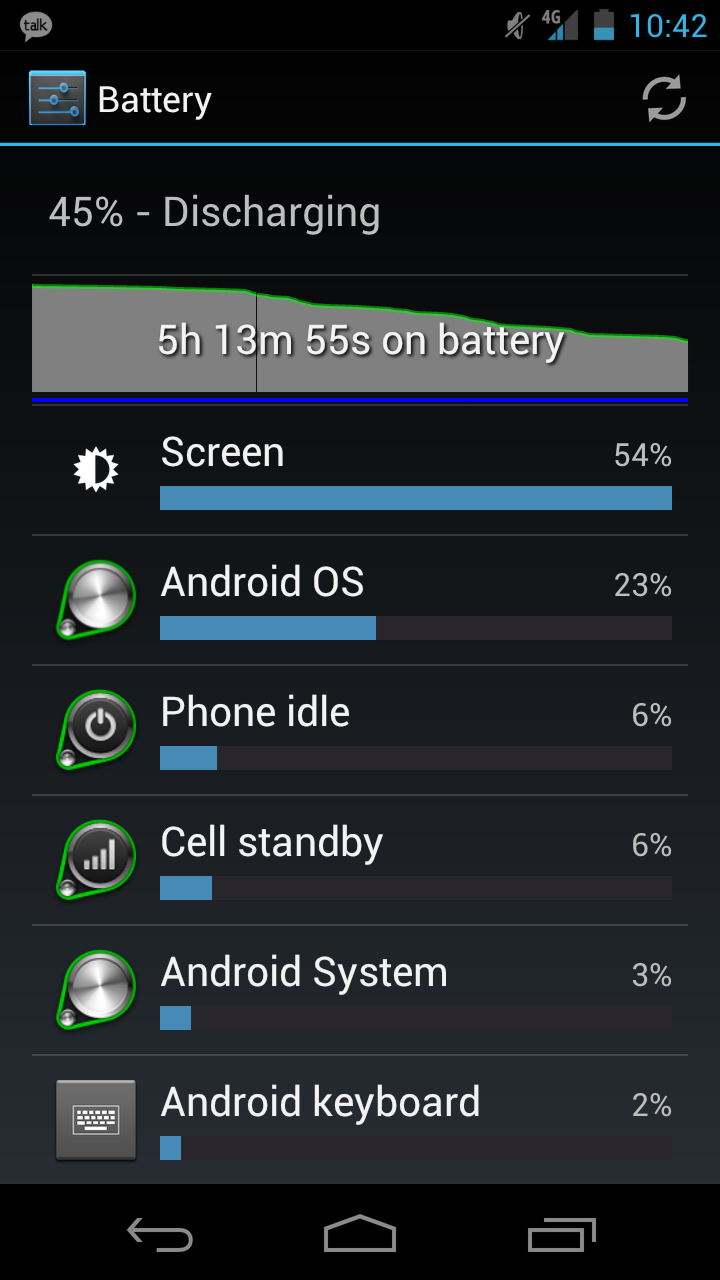
\includegraphics[scale=0.2]{figures/galaxy-nexus-battery.png}
	\end{center}
	
	\caption{Confirmation message on the FriendFinder app}.
	\label{pic:ff_conf}

\end{figure}

For the data to reach the database on the Google App Engine, an internet connection is required. However, the app can also function off-line, by saving all the data locally, and sending it to the on-line database as soon as an internet connection is established. It does this by using an IntentService \cite{intentservice}, which has two main functions:

\begin{itemize}
  \item A first function is to store the data locally, until an internet connection is established.
  \item the second, and most important, is to check periodically for an internet connections. Once an internet connection has been established, all the data is sent to the Google App Engine. The app checks every one minute for internet access. This allows for a relatively fast updating of the database, while at the same time keeping the resource use at a level that does not impede the normal functioning of the phone.
\end{itemize}

The data is stored locally in RAM of the phone (the volatile memory). This is made possible by the relatively small size of the data being saved ( the names of the two people involved, and an ID object that also serves as a timestamp) and the memory capacity of the phone ( approximately 700 MB of RAM). However, this has the disadvantage of being vulnerable to the phone turning off due to lack of battery. The volunteers have been made aware of this fact. 

Once the internet connection is established, the actual sending of the data is a simple matter, done with the help of the Google App Engine API. One thing to mention here is that each data entry is sent individually. If at any point, a \textit{save data} request is met by a \textit{failure} answer, the request is repeated until the \textit{success} message is received. In case of \textit{failure}, subsequent attempts have a one second delay between them. This is done to ensure that the app does not impede the overall functionality of the phone.



\subsection{Data}

Once a button with the name of a person is pressed, the data that is saved on the phone, and eventually sent and saved on the online database has the following format:

\begin{verbatim}
{ID, owner, target}
\end{verbatim}

\begin{description}
  \item[ID] It has a double role. First, the ID is a unique identifier, used for differentiating between multiple entries, as well as for various database operations. This field is required by the Google App Engine. Secondly, the ID also plays the role of the timestamp, used in future computations. While there are valid concerns that the ID might not be unique, due to two people pressing the button at the same time, the fact that the timestamp also includes the millisecond, and the fact that there are only three participants in the project results in an extremely low probability of identical timestamps. Obviously, the timestamp corresponds to the moment the button was pressed, and not the moment the data was sent to the database.  
  \item[owner] This field refers to the owner of the phone, which indicates the person that has made the observation.
  \item[target] This field names the person that has been observed by the owner.
\end{description}

Fig. \ref{pic:dataviewer} shows an example of how the data looks, with the caveat that the \textit{friend} field in the image corresponds to the \textit{target} field in the description above. The saved data was accessed and retrieved by API calls to the Google App Engine.  

\begin{figure}[h]
	\begin{center}
		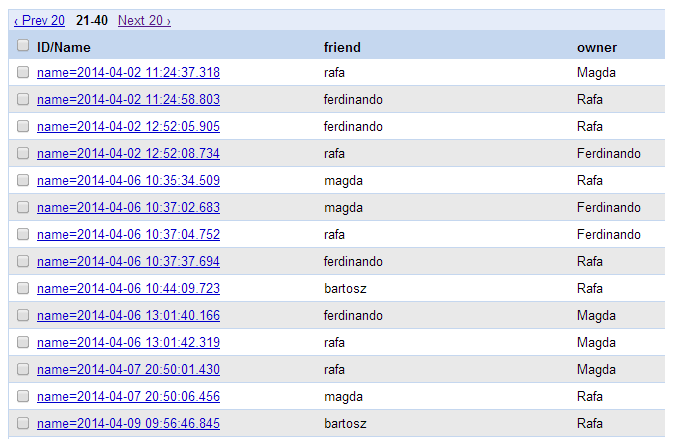
\includegraphics[scale=0.8]{figures/datastore.png}
	\end{center}
	
	\caption{Saved entries for the FriendFinder app}.
	\label{pic:dataviewer}

\end{figure}


\section{SensibleDTU data}

 The second type of data comes from the SensibleDTU data collector app. Based on \cite{Stopczynski,sensibledtu}, we will give a short description of the project, with an emphasis on data collection. We will then focus on the actual data, its form, and how it was collected. 

\subsection{Project overview}
 
 SensibleDTU is the implementation of a large scale study aimed at observing the various interchanges that take place between humans from a social and communications point of view. It aims to collect data on a large group of individuals, most of them students at DTU (Danish Technical University). The collected data consists of, among others, social relations and the networks that form as a result, geographical locations, and, of special interest to this thesis, face-to-face interactions. It does this by using a wide variety of sources, such as questionnaires, the wireless internet on campus, and mobile sensing through smartphones that were handed out to participants. A part of the data gathered through this last method is used in this thesis.
 
The smartphone data gathering is done by using a data collection app, based on the Funf framework \cite{funf}. This data is saved locally on the phone, and it is sent to a secure database server when the app detects the presence of an internet connection. Due to its sensitive nature, great care has been taken to ensure the privacy, security and anonymity of the saved data. Having said that, the three volunteers that participated in the data gathering for this thesis have agreed to the de-anonymization of their Bluetooth information, as it was required in order to merge the two sets of data gathered. 
 
 
\subsection{Data} 

The Bluetooth data is obtained periodically by the data collection app using the Bluetooth probe. Each phone performs a Bluetooth scan every five minutes. The scan lasts 30 seconds. While the 30 second scan lasts, the app saves all Bluetooth devices (that are discoverable) in its proximity, the time at which the scan has been made, as well as the RSSI \cite{vedran}. The data is stored on the phone from where it eventually reaches the secure database server, from where it can be downloaded. 

In order for the data to be used, it first needs to be \textit{cleaned}, as it contains additional meta-data ( fields used by the database for internal accounting), and devices that are not part of the study. The end result has the following format:

\begin{verbatim}
{timestamp, owner, target,signal_strength}
\end{verbatim}
 
 The above tuple has almost the same format as the one resulted from the FriendFinder app, with the addition of a new field, signal strength. At a first glance, one might think that the two sets of data can be easily combined. However, due to differences in the time when data gathering takes place, de-synchronization and the human factor, obtaining a single data set from the two is not a trivial matter. The following section goes into more detail regarding this issue.
 
\section{Data merger}

With the data merger we aim to obtain a single data set that consists of ordered entries of the following form, for each participant:

\begin{verbatim}
{timestamp, signal_strength, tag}
\end{verbatim} 

Where \textit{signal\_strength} refers to the RSSI, \textit{timestamp} refers to the timestamp provided by the SensibleDTU data collector app, and \textit{tag} is either \textit{yes} or \textit{no}. The \textit{tag} has the following meaning:

\begin{description}
  \item[yes] This tag means that the data has been confirmed through the use of the FriendFinder app. This means that we have co-location.
  \item[no] This tag mean that the data has not been confirmed through the use of the FriendFinder app. While the Bluetooth probe has discovered the device, and a RSSI exists, there is no co-location. The following are examples of situations where this might happen:  same room but a relatively large distance between the phones (cafeteria, large course rooms), transitional contacts (volunteers passing by each other), adjacent rooms with signal weakened by the walls. 
\end{description}

A first step is separating the SensibleDTU data on an user by user basis. For each volunteer, we obtain two timelines, which detail his interaction with the other two volunteers. Although measurements are taken every 5 minutes, the phones eventually become desynchronized. As such, we split the measurements into time windows, each window having a length of five minutes. This value was chosen because it matches with the period at which measurements are taken by the Bluetooth probe and gives a natural separation of the values obtained. Fig. \ref{pic:value_chain} shows a small part of a timeline with the splitting already done.

\begin{figure}[h]
	\begin{center}
		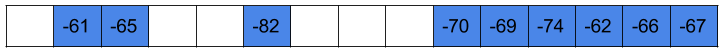
\includegraphics[scale=0.6]{figures/timechain.png}
	\end{center}
	
	\caption{Example of timeline for a single volunteer. The time windows are easily visible, as well as the RSSI value measured for each one. The values are expressed as \textit{dBm}.}
	\label{pic:value_chain}

\end{figure}

The above notion of tagging each timestamp now can be resolved by tagging each time window. The volunteers have been instructed to confirm the co-location once at the beginning of the meeting. In case of prolonged meetings, with separations and reunions, the volunteers were instructed to confirm again after each separation/reunion.   

In tagging the windows, we have used the notion of measurement chain. We define it as a continuous, ordered series of one or more time windows, where we have a RSSI value measured for every window in the chain. For example, in Fig. \ref{pic:value_chain} we have three distinct measurement chains: the first one with two windows, the second one with only one window, and the last one with six windows.

We tag a window \textit{w} with \textit{yes} if a FriendFinder app confirmation has been done in any window belonging to the chain that window \textit{w} also belongs, or the window immediately before, even if that window has no measurement. This last part is done to make sure that confirmations done in between Bluetooth probe measurements are not lost. Fig. \ref{pic:tag_yes} exemplifies how windows are tagged with \textit{yes}. 

\begin{figure}[h]
	\begin{center}
		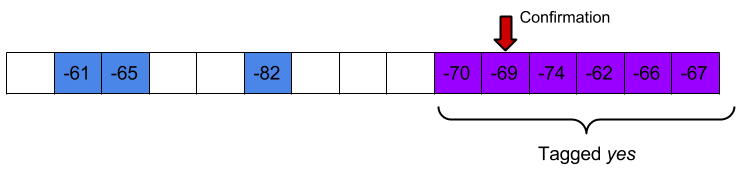
\includegraphics[scale=0.6]{figures/taggedyes.png}
	\end{center}
	
	\caption{Example of how tagging takes place as a result of a confirmation by FriendFinder app data.}
	\label{pic:tag_yes}

\end{figure}

After all the confirmations are taken into account and all the relevant chains are tagged with \textit{yes}, everything that remains is tagged with \textit{no}.  In the end we are left with a total number of 465 entries, Fig. \ref{pic:division} showing how they are divided: